\subsection{Devices connection}

\subsubsection{Android framework}
For Android framework, we used an initial \emph{connection setup phase} between devices.
Due to the implementation of \direct, devices cannot opportunistically create or destroy connections, so we were forced to manually create a \direct \textit{group} and provide devices with a complete address map in order to enable direct connectivity between all peers.

\begin{figure}[!htbp]
\centering
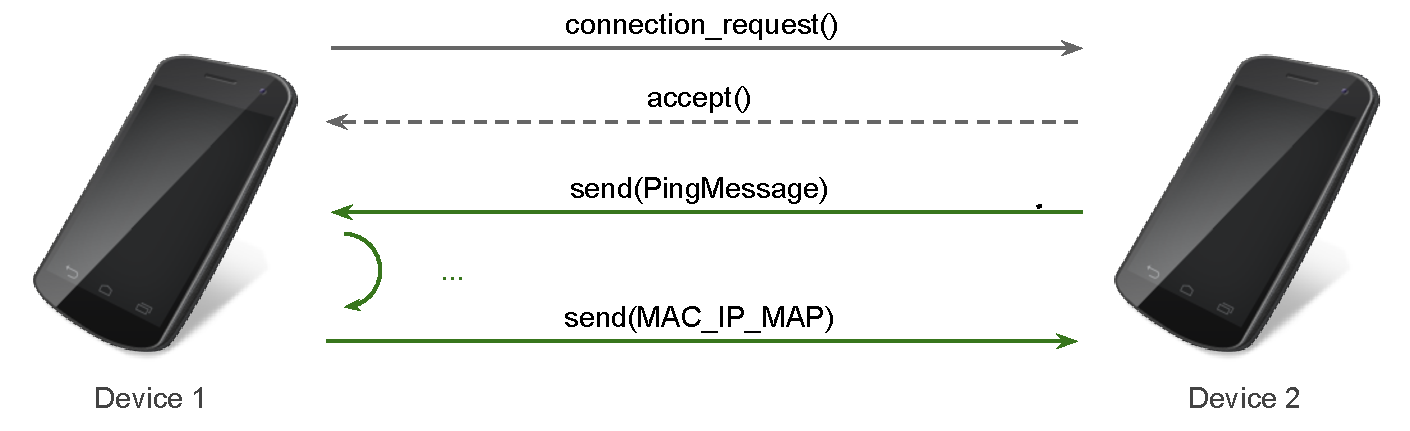
\includegraphics[width=3.6in]{imgs/device_connection_ops.pdf}
\caption{Connection operations sequence}
\label{fig:device_connection}
\end{figure}

The connection setup consists of the following operations:
	\begin{itemize}
		\item One of the devices asks other devices for connection
		\item When the request is accepted by a peer, a DHCP negotiation is started between the two. If no \direct group exists, it is created and the device which started the connection becomes the \textit{group owner}. If a group already existed, the accepting device is added to this group. At the end of this phase, each device has an IP address, but only the group owner's IP is available via \direct APIs. 
		\item Each device opens a \textit{TCP Server Socket} on port 8888, listening for incoming connections.
		\item When a device connects to a group, it sends a \textit{Ping message} to the \textit{group owner} via a socket. This kind of message is used by the \textit{group owner} to collect MAC and IP addresses of all devices in the group: the MAC address is included into the \emph{Ping message} by the sender device and the IP address is obtained by the receiver from the incoming Socket connection (using Java APIs).
		\item After collecting all the \begin{center}\tt{<MAC address,IP address>}\end{center} pairs from all the devices in the group, the \textit{group owner} creates a map and broadcasts it.
	\end{itemize}

Once these operations are concluded, all the devices are connected and can communicate between each other directly via TCP and UDP Sockets. An example of the obtained network is visible in figure \ref{fig:device_network}.

\begin{figure}[!htbp]
\centering
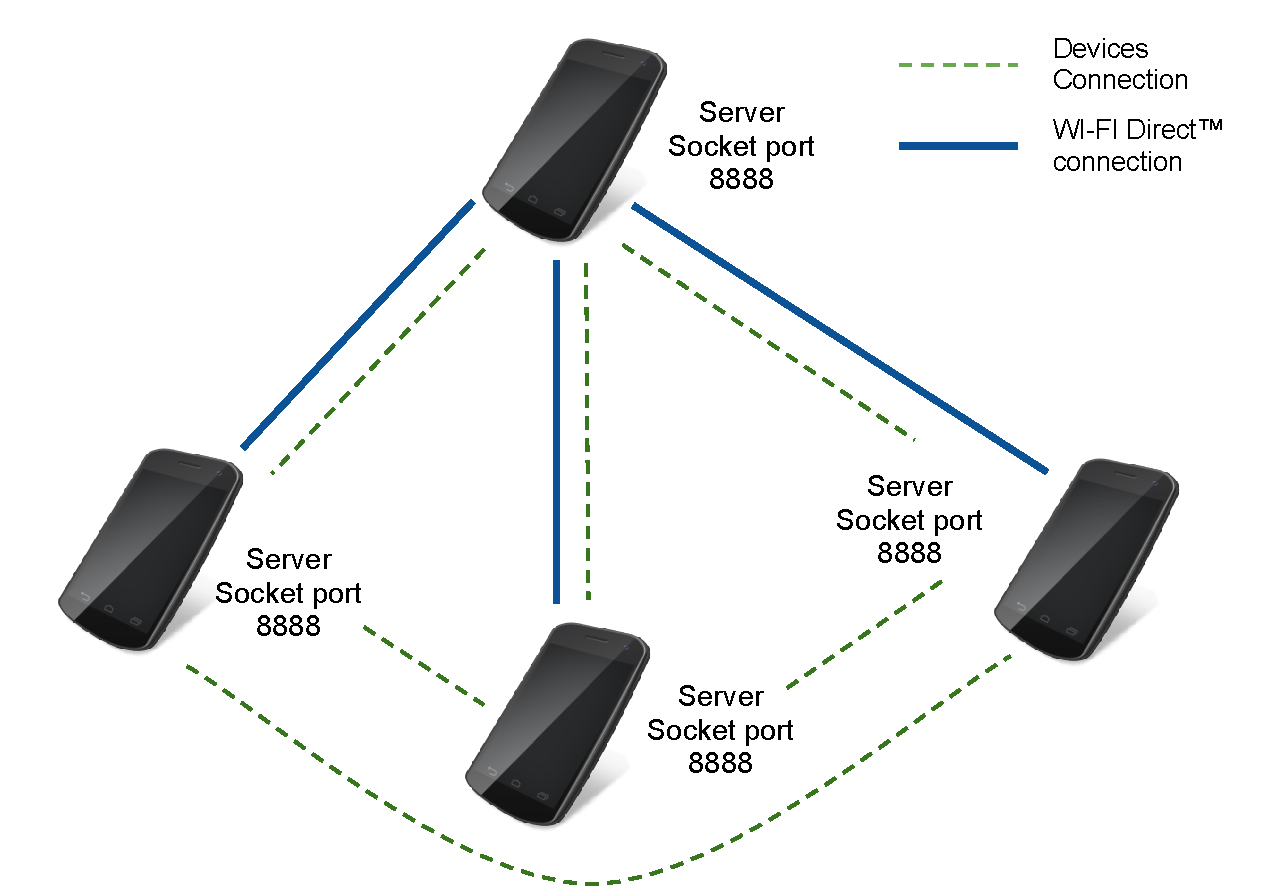
\includegraphics[width=3.6in]{imgs/Devices_network.pdf}
\caption{Network composed of four devices. Blu lines indicates the \direct group topology, and green lines the logical network}
\label{fig:device_network}
\end{figure}

\subsubsection{Desktop framework}
Although the used transmission protocol is completely connectionless and stateless (it only relies on Broadcast messages on the MAC Address FF:FF:FF:FF:FF:FF), an initial setup is needed to read the positions from the location file. More specifically, since the location file is unique for all of the instances of an application built on top of the framework, a mechanism to coordinate the reading is needed. To obtain this, before starting the simulation a random peer (called from now on \textit{master peer} for convinience) sends a \textit{StartSetup} message, and all other peers replies with a ping containing an unique \textit{Application ID} (a random number between 0 and \textit{INT\_MAX}; this is due to the fact that more instances of the application can run simultaneously on  the same machine, so nothing static like MAC Address could be used) whitin a 5 seconds window. Once the window is over, the \textit{master peer} assigns a progressive number to each peer and broadcasts a message containing a map \textit{\textless PeerID\textgreater\textless Progressive\textgreater} to coordinate the reading.
